\documentclass[reprint,amsmath,amssymb,aps, prl,superscriptaddress]{revtex4-2}
\usepackage{graphicx}% Include figure files
\usepackage{dcolumn}% Align table columns on decimal point
\usepackage{bm}% bold math
\usepackage{amsmath}
\usepackage{natbib}
\usepackage{chngcntr}
\usepackage{url}
\usepackage{float}
\usepackage{fourier} 
\usepackage{array}
\usepackage{makecell}
\usepackage{background}
\usepackage[english]{babel}
\usepackage[utf8]{inputenc}
\usepackage{fancyhdr}

\pagestyle{fancy}
% \fancyhf{}
\rhead{Lab-C (TAU)}
\lhead{Molecular Spectroscopy}

\bibliographystyle{apsrev}

\setcounter{tocdepth}{5}
\setcounter{secnumdepth}{5}
\renewcommand\theadalign{bc}
\renewcommand\theadfont{\bfseries}
\renewcommand\theadgape{\Gape[4pt]}
\renewcommand\cellgape{\Gape[4pt]}
\backgroundsetup{
   scale=1,
   angle=0,
   opacity=1,
   color=black,
   contents={\begin{tikzpicture}[remember picture, overlay]
      \node at ([yshift = -1cm] current page.north)
            {
\includegraphics[width = 3cm]{Images/logo.png}}; %
     \end{tikzpicture}}
}
\begin{document}

\preprint{APS/123-QED}

\title{Plastic, Air, Alcohol And Cigars\\Through The Lens Of An IR Spectrometer}
% Add Tau Logo


\author{Alon Shaaltiel}
\author{Oren Kereth}
\affiliation{Raymond and Beverly Sackler School of Physics and Astronomy, Faculty of Exact Sciences, Tel Aviv University, Tel Aviv 69978, Israel}
\author{Georgi Gary Rozenman}
\affiliation{Raymond and Beverly Sackler School of Physics and Astronomy, Faculty of Exact Sciences, Tel Aviv University, Tel Aviv 69978, Israel}
\affiliation{School of Electrical Engineering, Iby and Aladar Fleischman Faculty of Engineering, Tel Aviv University, Tel Aviv 69978, Israel}



\date{\today}% It is always \today, today,
             %  but any date may be explicitly specified

\begin{abstract}
Using FTIR and ATR spectroscopy we study the characteristics of gases, liquids and solids. When a light beam passes through a sample, certain wavelengths are absorbed depending on the sample's properties, thus allowing us to analyze the sample based upon its IR spectrum. Polyester's refractive index is found from thin film interference, alcohol concentrations in drinks are calculated, the molecular constants of carbon-monoxide are found and the ratio of carbon-dioxide in exhaled air compared to fresh air worryingly shows a downward trend through the years. Lastly, chemical products in various cigars' smoke are identified and a comparison between the cigars based on the toxicity of their contents is made.
\end{abstract}

%\keywords{Suggested keywords}%Use showkeys class option if keyword
                              %display desired
\maketitle
\renewcommand*{\thesection}{\arabic{section}}
\renewcommand*{\thesubsection}{\arabic{section}.\arabic{subsection}}
% \renewcommand{\thefigure}{\arabic{figure}}

\section{Introduction}
In this experiment the Fourier Transform Infra Red spectrometer (FTIR) will be used extensively to extract the infra-red spectrum of various materials and compounds. The infra-red spectrum consists of the intensity of incoming light made out of a range of wavelengths transmitted through a sample. The sample absorbs some wavelengths thus yielding an IR spectrum of that particular sample.
% We never said what IR is outside of FTIR. re: added

A short historical overview is presented for the reader, for more information see References.
% Change to "A short historical overview is presented for the reader, for more information see References." re: changed
In 1800 IR was recognized as a distinct region of the energy spectrum by Sir William Herschel, however the study of IR light with various materials started about 100 years later. In 1903, William W.Coblentz measured the IR spectra of hundreds of inorganic and organic compounds\cite{scitool}.
% Why did he measure them? re: no idea, wasn't written
As a result of increasing interest in the field, the first prototypes of IR spectroscopy were built in the 1930s.  In 1949 the astrophysicist Peter Fellgett used an interferometer to measure light from celestial bodies and produced the first Fourier transform infrared spectrum, however this method was still limited and took many hours to compute. In the late 1960s, commercial FTIR spectrometers appeared as
% because sounds less scientific than as. re: ok
microcomputers were able to do the Fourier transform, however
% maybe say "contrary to what the name suggests, they were..." re: 'i don't know about that
they were large and expensive. Over time, technology reduced the costs and size,
% size? re: ok
increased availability and enhanced the capabilities of FTIR spectroscopy systems\cite{spechistory}.


\subsection{Thin Film Interference}
Upon contact with a beam of light, the internal reflections in a thin sample of material with a sufficiently high refractive index are not negligible.
\begin{figure}[H]
    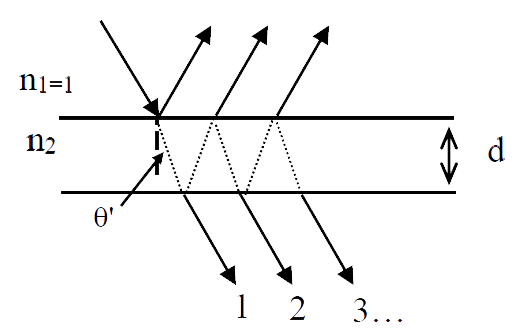
\includegraphics[width=\linewidth]{Images/Thin film.png}
    \caption{Reflected and transmitted light waves from a thin film}
    \label{fig:ThinFilm}
\end{figure}
This experiment concerns only the transmitted beams; The treatment for reflected beams is quite similar.\\
In this experiment only the intensity of the beams is detected, to understand how coherent light beams with the same wavenumber, $\vec{k}$ (and frequency, $\omega$) affect the detected intensity, an example of two beams is given. 
The electric fields, $\vec{E}$, of the two beams are
\begin{equation*}
    \vec{E_{i}}=E_{i}e^{i(\omega t - \vec{k}\cdot\vec{r} + \varphi_i)}\hat{\epsilon}_1;\ i=1,2
\end{equation*}
% Should "I "write what everything represents?
where $\varphi_i$ is the electromagnetic wave's phase shift and $\hat{\epsilon}_1$ is the polarization.
The detectable wave is the super-position of both waves
\begin{equation*}
    \vec{E} = (E_{1}+E_{2}e^{i\Delta\varphi})e^{i(\omega t - \vec{k}\cdot\vec{r} + \varphi_1)}\hat{\epsilon}_1;\ \Delta\varphi=\varphi_2-\varphi_1
\end{equation*}
An electromagnetic wave's intensity is proportional to $|\vec{E}|^2$ thus, the detected intensity is proportional to 
\begin{equation*}
\begin{split}
    |\vec{E}|^2 = E_{1}^2 + E_2^2 + \Re\{2E_{1}E_{2}e^{i\Delta\varphi}\}\\ \rightarrow I=I_1+I_2+2\sqrt{I_1I_2}cos(\Delta\varphi)
\end{split}
\end{equation*}
If $\Delta\varphi=2n\pi;\ (n\in\mathbb{Z})$, $I$ is at its maximum, this is called "constructive interference". If $\Delta\varphi=(2n+1)\pi;\ (n\in\mathbb{Z})$, $I$ is at its minimum, this is called "destructive interference". If $\Delta\varphi$ is changed linearly the detected intensity would result in a cosine$\backslash$sine\cite{FundamentalsOfPhotonics}.\\
Now onto the transmitted beams, the phase between two consecutive transmitted beams and relative intensity are
% ADD REFRENCE
% NOTICE ME 
\begin{equation} \label{eq:ThinPhaseAmp}
\Delta\varphi=k(2n_{2}dcos\theta)
\end{equation}
where $k=\frac{2\pi}{\lambda}$ is the beam's wave number, $\lambda$ is the beam's wave length, $n_{2}$ is the sample's refractive index, $\theta$ is the beam's angle inside the sample and d is the sample's thickness. $2n_{2}dcos\theta$ is the optical path length (OPL) difference. Constructive interference occurs if $\text{OPL}=\frac{m}{k}$ and if $\text{OPL}=\frac{m+\frac{1}{2}}{k}$, destructive interference occurs, where $m\in\mathbb{Z}$. The difference in wavenumber ($\Delta k$) between two destructive peaks of intensity would be (Equation \ref{eq:ThinPhaseAmp})
\begin{equation} \label{eq:ThinDiffWavenum}
\Delta k=\frac{1}{2n_{2}dcos(\theta)}
\end{equation}

% By measuring both $\Delta k$ using a Fourier transform of the intensity or a sine fit, and the thickness of the sample in the lab, the material's refractive index can be extracted 
% \begin{equation} \label{eq:ThinRefractIndex}
% n_2=\frac{1}{2\Delta kdcos(\theta)}
% \end{equation}

\subsection{The Beer-Lambert Law}
The Beer-Lambert Law describes how a monochromatic beam of light is absorbed in relation to substance concentration. The dependency is given by
\begin{equation} \label{eq:BeerLambert}
\text{ln}\left(\frac{P(v)}{P_{0}(v)}\right)=A=-av_{\alpha\alpha'}Cx
\end{equation}
where $P(v)$ is the light's intensity through the sample, $P_{0}(v)$ is the intensity with no sample, $A$ is the absorbance, $a$ is the molar attenuation coefficient, $\alpha$ and $\alpha'$ are quantum numbers, $C$ is the concentration, and $x$ is the optical path length of the beam, given by $n\cdot l$ where $l$ is the distance the beam traveled and $n$ is the material's refractive index. All else being equal, the absorbance and concentration are proportional to one another. \\
The Beer-Lambert Law does have its limitations, for starters, it is only valid for low concentrations, according to (\Citeauthor{2020Beer}, \cite{2020Beer}) at higher concentrations "the individual particles of analyte no longer are independent of each other", this may change the material's absorptivity. On top of that, at high concentrations a solution's refractive index may change across concentrations \cite{2020Beer}.

\subsection{CO Molecule IR Spectrum}
The model used to describe CO molecules
% either write "a CO molecule" or just shorten to "The model used to describe diatomic molecules..." re: agreed
and other diatomic molecules pictures a molecule in which the individual atoms, held together by chemical bonds, are in vibratory motion along these bonds, while the molecule as a whole is rotating \cite{alpert}. The energy states of this system correspond to a Hamiltonian with a potential 
% maybe add a H = ?? + V; V=... to the equation to make it more readable? re: I'm not entirely sure.
\begin{equation} \label{eq:CO_Potential}
V(\boldsymbol{r})=\frac{1}{2}k(r-r_0)^2
\end{equation}
and can be expressed as a combination of rotational and vibrational energies
\begin{equation} \label{eq:CO_RotVibEnrg}
E=E_{Rot}+E_{Vib}= hcw_{e}(\nu +\frac{1}{2}) + \frac{\hbar  ^2}{2I}J(J+1)
\end{equation}
where $h$ is Planck's constant, $\hbar$ is the reduced Planck's constant, $c$ is the speed of light, $w_{e}$ is the wave number corresponding to the frequency of vibrations, $\nu$ is a quantum number corresponding to the vibrations,  $I$ is the molecule's moment of inertia and $J$ is a quantum number corresponding to the angular momentum of the particle \cite{griffithsQM}. However, the  current potential is not truly harmonic and only serves as an approximation,
% "However, this is only an approximation" may sound better re: integrated it into the text now
as effects such as the centrifugal force, Coriolis and Fermi \cite{alpert} require the use of perturbation theory \cite{samurai}. Using the perturbation theory, the energy states are now
% now is unnecessary IMO re: Wanted to elaborate a little more and also add a reference.
\begin{equation} \label{eq:CO_PeturbRotVibEnrg}
\begin{split}
& T=T_{Vib}+T_{Rot}=\\
& w_{e}(\nu +\frac{1}{2}) -w_{e}x_{e}(\nu +\frac{1}{2})^2+ \\
& B_{v}J(J+1)-D_{v}J^2(J+1)^2 
\end{split}
\end{equation}
where $x_{e}$, $B_{v}$ and $D_{v}$ are constants which take into account small perturbations and $T$ is the energy states in wave number units ($T=\frac{E}{hc}$
% isn't it h-bar? re: no, in theory its h
). At room temperature only the $\nu=0$ state is occupied while the $J$ states are all occupied. Therefore, using selection rules \cite{griffithsQM} only the transitions $\nu$ $\rightarrow $ $\nu'$  where $\nu ' =1,2,3$  and $J$ $\rightarrow $ $J'$ where $J'=J+1,J-1$   are of interest. Using equation \ref{eq:CO_PeturbRotVibEnrg}
% notice  re: thanks, forgot about it                ^^^^^^^^^^^^^^^^^^^^^^^^^^^^^^^^^^^^^^^^^^^^^^^^^^^
the allowed spectral lines are derived to be
\begin{equation} \label{eq:CO_DiffPeturbEnrg}
\begin{split}
& \Delta T =T(\nu ',J')-T(0,J)=\\
& w_{e}\nu' -w_{e}x_{e}(\nu'^{2})+(2B_{e}-\alpha(\nu'+1))m-\\
& \alpha\nu'm^2-4D_{v}m^{3}
\end{split}
\end{equation}
where $\Delta T$ is the allowed spectral line, $B_{e},\alpha $ are constants related to $B_{v}$  which are the result of further corrections due to perturbation theory and $m$ is either $J+1$ or $-(J-1)$  depending on the transition. In this experiment the transitions to $\nu'=1$ and $\nu' =2$ will be of interest, for which $\Delta T=2141cm^{-1}$ and $\Delta T = 4255 cm^{-1}$ respectively.


\section{Experimental System and Measurements}
There are two main measuring instruments in this experiment- FTIR and ATR. Both use Michelson interferometers and perform a Fourier transform.

\subsection{Michelson Interferometers}
A Michelson interferometer consists of two perpendicularly plane mirrors, one of which can travel in a direction perpendicular to the plane.
% maybe say "can travel in and out" while less scientific per se, it's more clear. RE: I agree that it can be more clear that way, but the figure helps in understanding it. if you think otherwise I'll change it. 
A semi reflecting film, the beamsplitter, bisects the planes of these two mirrors. The beamsplitter splits the beam into two, one beam transmitted through the beamsplitter and the other reflected from it. Both beams then get reflected from the mirrors, returning to the beamsplitter where they recombine and interfere \cite{stuart} (see Figure \ref{fig:Interferometer}). 
% needs reference re: fixed
\begin{figure}[H]
    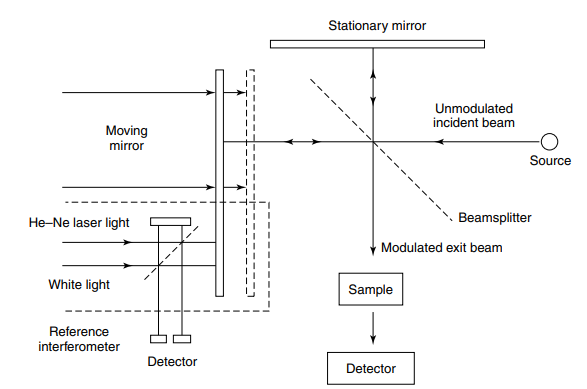
\includegraphics[width=\linewidth]{Images/INTERFEROMETER.png}
    \caption{Schematic of a Michelson interferometer \cite{stuart}.}
    \label{fig:Interferometer}
    \centering
\end{figure}
The beam which emerges from the interferometer at 90 degrees to the input beam is called the transmitted beam and is the beam detected by the detector as can be seen in Figure 2.
% "the beam detected by the detector" to "the detected beam" re: this was the first time I mentioned the detector.
The moving mirror produces an optical path difference between the two split beams.
% "between the two beams split by the beamsplitter" to "between the two split beams" re: fixed
Plotting the signal produced by the detected beam
% maybe change to "the beam's intensity" re: 'i don''t know, signal sounds more intuitive 
as a function of the change of
% (optical)
optical path length between the two beams yields
% "will yield" to "yields" ? re: fixed
an interferogram. By performing a Fourier transform on the interferogram the spectral distribution of the beam (i.e. the amplitude of each wave number the light is made of.)
% "is consisted of" to either "consists of" or "is made of re: fixed
can be found.

\subsection{FTIR}
FTIR stands for Fourier Transform Infra-Red spectrometer.
% (spectrometer) and maybe capitalise the T and I, maybe take "infrared" to "Infra Red" to make it even clearer re: fixed
IR radiation is passed through a sample.
Some
% I think LTex is right, prolly remove the "Some of" re:fixed 
infrared radiation is absorbed by the sample and some of it is
passed through (transmitted). The resulting spectrum represents the molecular
absorption and transmission \cite{FTIRmanual}. FTIR (see Figure 3) utilizes Michelson interferometers, the interferogram and a Fourier transform to perform the analysis of the spectrum. 
\begin{figure}[H]
    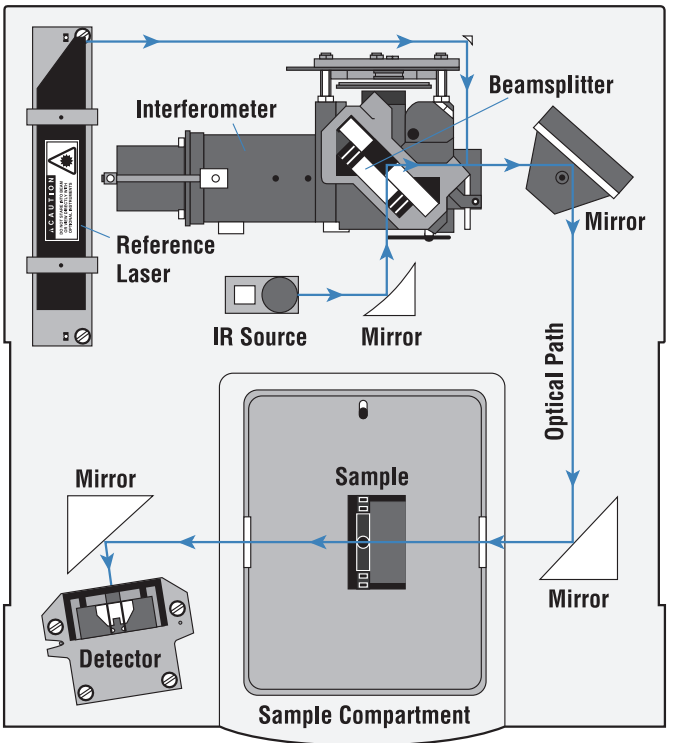
\includegraphics[width=\linewidth]{Images/FTIR LAYOUT.png}
    \caption{Layout of the FTIR spectrometer \cite{FTIRmanual}.}
    \label{fig:FTIR}
    \centering
\end{figure}

As can be seen in Figure \ref{fig:FTIR}, a black-body source emits IR radiation. The radiation then passes through an interferometer, where the 'spacial encoding' takes place \cite{FTIRmanual}. A He-Ne laser is used as a reference for calibration of the moving mirror's position \cite{stuart}. After going through the interferometer, an interferogram is created. The interferogram then passes through the sample, where specific wave numbers are absorbed according to the sample's characteristics and the rest are transmitted into the detector where the interferogram signal is measured. The data reaches the computer, which performs a Fourier transform yielding the infrared spectrum consisting of absorption lines corresponding to the sample. 

\subsection{ATR}
ATR, which stands for \emph{Attenuated Total Reflection}, measures the absorbance of a liquid or solid using IR spectroscopy. A crystal with a sufficiently high refractive index to achieve total internal reflection is surrounded by the material whose absorbance is of interest. 
\begin{figure}[H]
    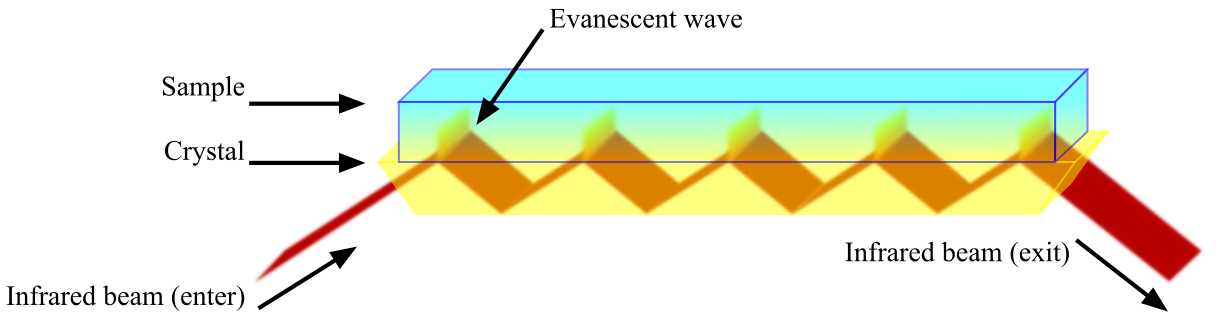
\includegraphics[width=\linewidth]{Images/ATR.png}
    \caption{Layout of an ATR compartment \cite{wiki:ATR}}
    \label{fig:ATR}
    \centering
\end{figure}
An interferogram is projected into the crystal and evanescent waves, resulting from the total internal reflection, propagate through the sample. 
% Evanescent waves, similarly to most waves are a product of an amplitude and an exponent: $|\vec{E}|=Ae^{i(\omega t - \vec{k}\cdot\vec{r})}$, however, unlike most EM waves, evanescent waves have a complex $\omega$ (and $|\vec{k}|$). Separating $\omega$ and $\vec{k}$ to their Real and Imaginary parts and choosing $\vec{k}$'s direction as $\hat{z}$ yields
% \begin{equation}
%     |\vec{E}|=Ae^{i(\omega_R t - k_{R}z)}e^{-(\omega_I t + k_{I}z)}
% \end{equation}
Evanescent waves penetrate the sample with an exponentially decreasing amplitude and intensity with distance.
When no sample is inserted, and a vacuum surrounds the crystal, the energy evanescent waves carry is wholly returned $\langle\frac{dU_{Eva}}{dt}\rangle=0$. However, if a sample is inserted into the ATR, and evanescent waves propagate through it, wave-lengths corresponding with the sample's normal modes are absorbed and the energy of the reflected beam decreases $\langle\frac{dU_{Eva}}{dt}\rangle<0$. As described in the previous paragraph, the interferogram is detected and disassembled into the sample's infrared spectrum.

\subsection{Transmission Through Thin Films of Polyester}
In this part of the experiment the refractive index of a thin sample of polyester is extracted. Thin polyester samples with varying widths are placed in the sample area perpendicular to the beam's direction. An interferogram is projected through each sample. The resulting IR absorbance spectrum will be a summation of the material's (polyester's) absorbance spectrum and the sine wave showing absorption from thin film interference. To extract the frequency of destructive interference ($\frac{1}{\Delta k}$ in eq. \ref{eq:ThinDiffWavenum}) a sine wave is fitted to the region in the absorbance spectrum with the clearest sine wave, the fit's frequency is taken as the sample's frequency. Using equation \ref{eq:ThinDiffWavenum}, the extracted sine frequency, the measured width, and $\theta=\frac{\pi}{2}$, as the sample is perpendicular to the beam, a fit of the form
\begin{equation}
    \begin{gathered}
        \label{eq:ThinLinFit}
        d=a_{0}+a_{1}f_{fit} \\
        f_{fit} = \frac{1}{\Delta k};\ a_1=2n_{2};\ a_0\approx 0
    \end{gathered}
\end{equation}
was made. Some samples' widths were not measured and only had an interferogram projected through them. By fitting a sine to their IR spectra and inputting their fitted frequency into the calibrated relation in equation \ref{eq:ThinLinFit}, their widths can be approximated.

\subsection{Calibration Using Ethanol} 
In this part of the experiment the relationship between the concentration of a dissolved substance inside a solution
% , re: where?
to its total absorbance amplitude, which is assumed to be linear according to equation \ref{eq:BeerLambert}, was calibrated. The calibration was done using solutions of water and ethanol  with varying known concentrations. The solution was put into a tank inside an ATR. Starting from a concentration of $96\%$, the ethanol was diluted by adding more water into the solution, thus changing the concentration of the ethanol according to 
\begin{equation} \label{eq:EthanolConcentrVolume}
C_{i}V_{i} = C_{f}V_{f}
\end{equation}
where $C_{i}$,$V_{i}$, $C_{f}$,$V_{f}$ are the initial and final concentration of ethanol and volume of the solution respectively. The final measurement was at a 40\% concentration of ethanol.
For each concentration, $C$, the total absorbance of the solution in the range $1000-1120cm^{-1}$, $F$, was calculated. In this range lie the absorption peaks of ethanol \cite{NISTwebook} and therefore, according to equation \ref{eq:BeerLambert} their intensity is proportional to the concentration of ethanol in the solution. A calibration graph of the form 
\begin{equation} \label{eq:EthanolLinFit}
    C=a_{0}+a_{1}F 
\end{equation} 
was then made. Using the calibration, the concentration of different solutions was found by calculating their total absorbance, F. 

\subsection{$\text{CO}_{2}$ and IR Spectrum of CO}
Using a pump, exhaled and room air were each inserted into a chamber in the FTIR. For each of the two types of air the total absorbance in the range $2270-2400cm^{-1}$ was
% was re: fixed
calculated. In this region there are two absorption peaks both corresponding to the concentration of $\text{CO}_{2}$ in the air. The ratio between the total absorbance of the exhaled air to the room air in that region, denoted by $S$ is therefore equal to the corresponding ratio between $\text{CO}_{2}$ concentrations in each of them. $S$ will then be compared to previously measured ratios. 
% "ratios previously measured" to "previously measured ratios" re: fixed
Afterwards, by pumping CO into to the same chamber in the FTIR, its IR spectrum was measured.
% I don't think "and" is supposed to be there re: fixed
According to equation \ref{eq:CO_DiffPeturbEnrg}
% need to reference re: fixed
the spectrum contains absorption peaks that represent a transition in the angular momentum of the molecule, $J$  to either $J+1$ or $J-1$ (see Figure \ref{fig:CoEnergy}).
% need to reference re: fixed
\begin{figure}[H]
    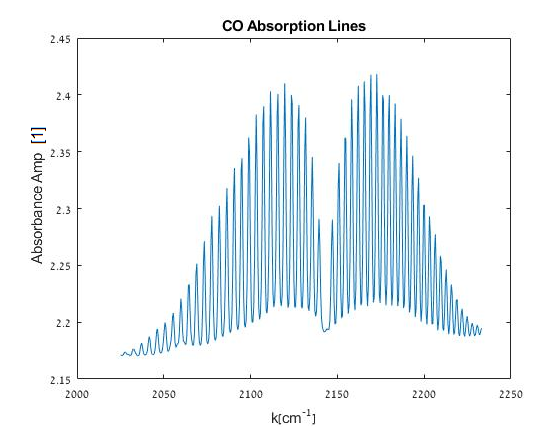
\includegraphics[width=\linewidth]{Images/COEnergystatesUPDATED.png}
    \caption{CO absorption lines in the region $2025-2233 cm^{-1}$. Each peak represents a transition $m$ of the angular momentum and the transition from $\nu=0$ to $\nu'=1$ which is centered at 2141$cm^{-1}$  as can be seen and according to subsection 1.3.
    % need to reference
    }
    \label{fig:CoEnergy}
    \centering
\end{figure}
Each of the peaks, $m$, were numbered according to its order relative to the center point at 2141$cm^{-1}$ (i.e. if $m$ was the first to its left
% what's "its" (I know you're talking about the center of the mustache but it's pretty unclear), writing "to the left" instead of "to its left" is also clearer if you'd prefer that
it was numbered as $-1$ and if it was the first to its right
% same as last comment
it was numbered as $1$). Afterwards, a polynomial fit of $3^{rd}$ order was made between $\Delta T$ and $m$ from equation \ref{eq:CO_DiffPeturbEnrg}
% need to reference
\begin{equation} \label{eq:CO_EnrgStatesFit}
    \Delta T = a_{0}+a_{1}m+a_{2}m^2+a_{3}m^3
\end{equation}
The coefficients extracted from the fit will then be used to extract the coefficients in equation \ref{eq:CO_DiffPeturbEnrg}
% need to reference re: fixed
according to the relations 
\begin{equation}
\begin{aligned}
\alpha &=-a_{2} & D_{v}&=-\frac{a_{3}}{4} & w_{e}&=2a_{0}-\frac{4255}{2} \\
B_{e}&=\frac{a_{1}-2a_{2}}{2} &  x_{e}&=\frac{a_{0}-\frac{4255}{2}}{2a_{0}-\frac{4255}{2}}
\end{aligned}
\label{eq:COFITcoefficients}
\centering
\end{equation}
where in order to find $w_{e}$ and $x_{e}$ the spectral line, $\Delta T=4255 cm^{-1}$, of the transition $\nu =0 \rightarrow \nu'=2$ and $\Delta J =0$ was used. The extracted values of the coefficients will then be compared to their corresponding theoretical values.

\subsection{IR Spectra of Different Cigar Brands}
In this part of the experiment gases in the smoke of various cigars are analyzed. An interferogram is projected through regular air. A pump smokes on a cigar and fills the sample area with smoke. An interferogram is projected through the smoke and the absorbance spectrum compared to regular air is created. Various toxic gases are identified. Each gas's total absorption (TA) was calculated using trapezoidal rule \cite{numerical} and taken as a proxy to concentration. The TA of different substances cannot be compared; However, the TA of the same substance in different cigar brands can be directly compared. The comparison will look at the different substances and relative quantities and try to answer which is the most harmful.
% Maybe correct the concentration claim

\section{Results}

\subsection{Polyester Refractive Index Calculation}
For each sample width the area with the clearest sine wave in the absorption spectrum was found and fitted to a sine wave.
\begin{figure}[H]
    
    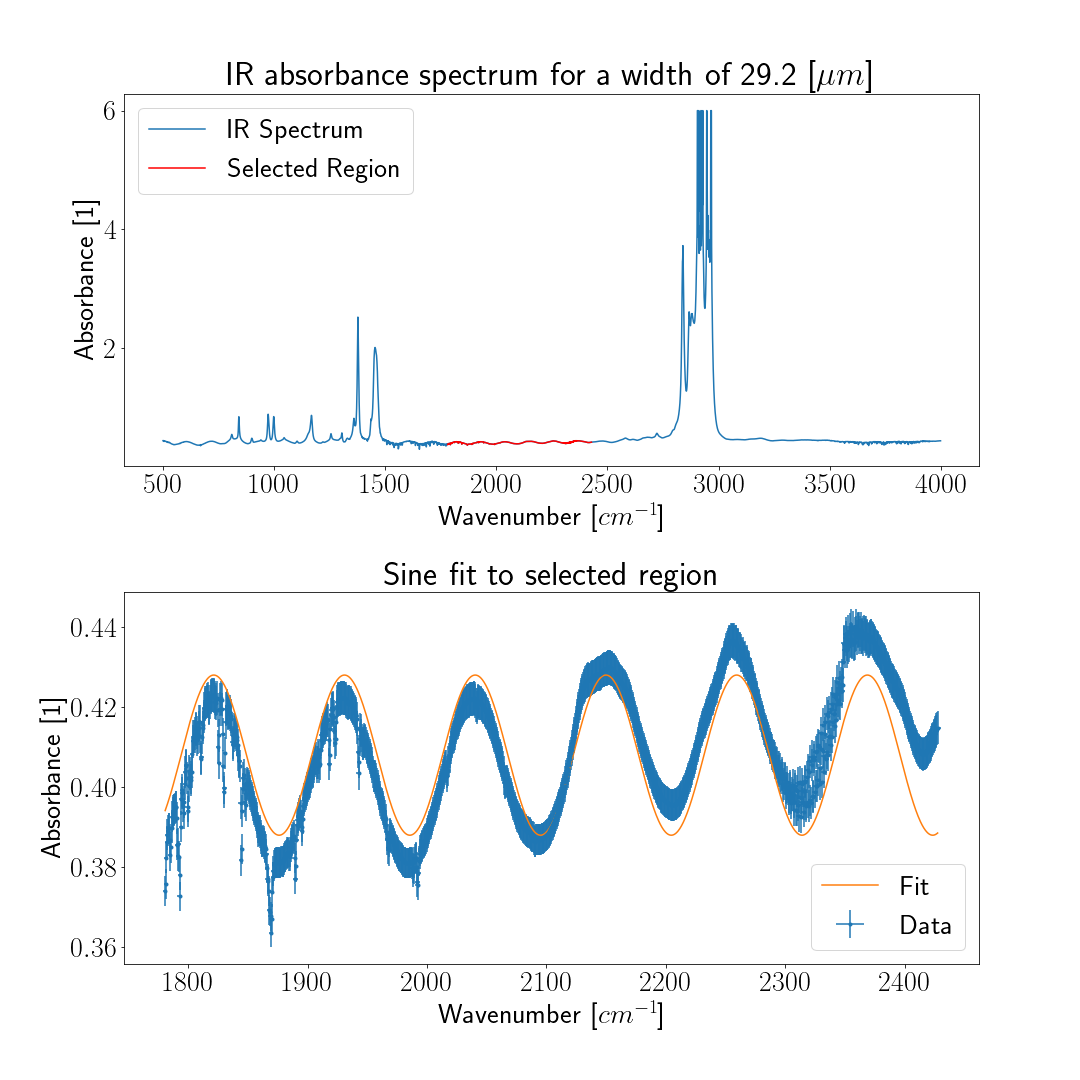
\includegraphics[width=\linewidth]{Images/29_2_Spec.png}
    \caption{IR absorbance spectrum and sine fit to the selected region for a width of $29.2\ [\mu m]$}
    \label{fig:SineFitEx}
    \centering
\end{figure}
Fitting a linear function between the width and the frequency of the associated sine (eq. \ref{eq:ThinLinFit}) yielded the following (See Figure \ref{fig:ThinLinWidthFreq})
\begin{figure}[H]
    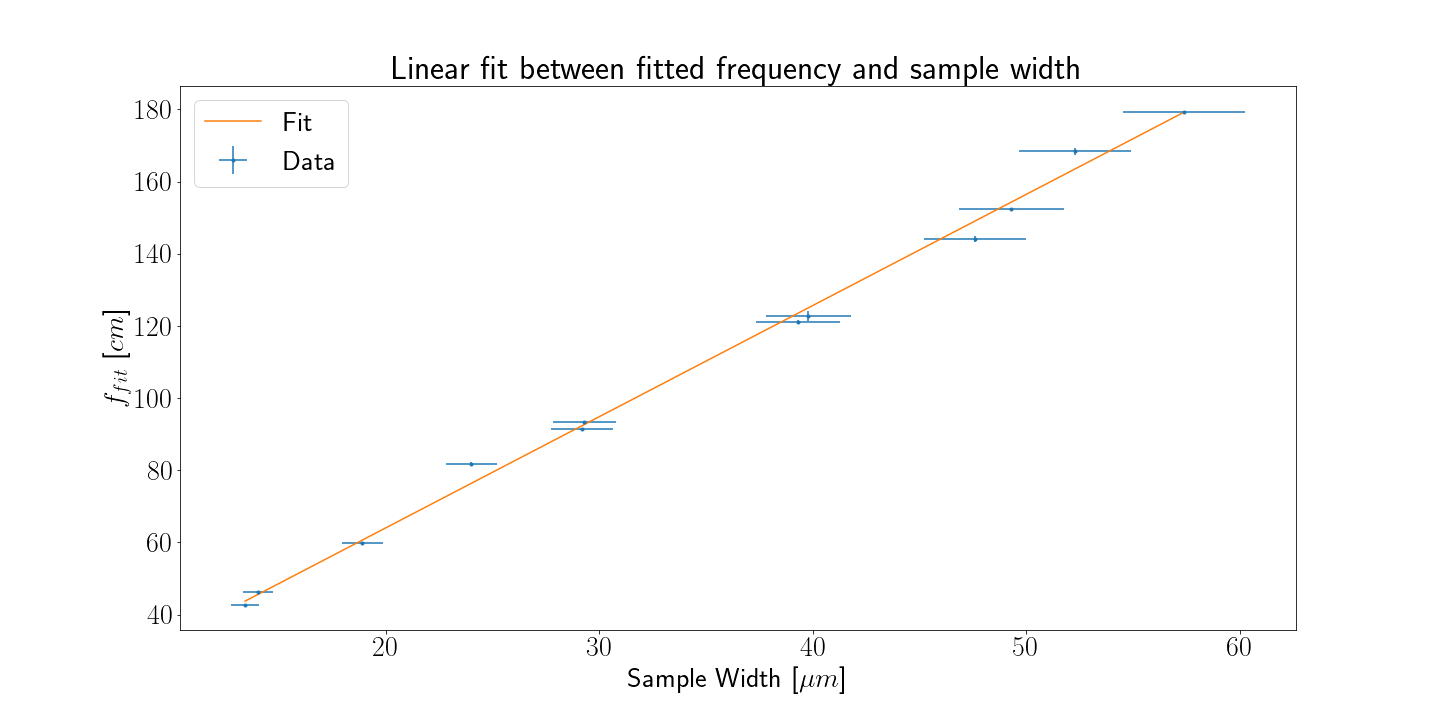
\includegraphics[width=\linewidth]{Images/__linear_fit.png}
    \caption{Linear fit between the fitted frequency, $f_{fit}$, and the sample width.}
    \label{fig:ThinLinWidthFreq}
    \centering
\end{figure}
The fit's statistical measures are $P_{value}=0.95$ and $\chi^2_{red}=0.39$, both suggest a slight over-estimation of errors.
The fit parameters of the linear fit can be seen in Table \ref{tbl:WidthFit}
\begin{table}[H]
    \centering
    \begin{tabular}{ |p{2cm}|p{2cm}|p{3.3cm}|  }
     \hline
     \multicolumn{3}{|c|}{\thead{Fit Parameters of Width vs. Frequency}} \\ \hline
     Parameter & Value & Error (Relative Error)\\ \hline
     $a_{0}$[$cm$]  &$2.4$      &$1.5$ ($60\%$) \\ 
     $a_{1}$[$1$]   &$3.080$    &$0.060$ ($1.9\%$)  \\ \hline
    \end{tabular}
    \caption{Fit parameters of the sample width vs. fitted frequency fit}
    \label{tbl:WidthFit}
\end{table}

Using equation \ref{eq:ThinDiffWavenum}, the extracted refractive index is
\begin{equation}
    n = \frac{a_1}{2} = 1.540 \pm 0.030\ \text{[1]}
\end{equation}
Using the calibrated correlation between sample width and sine frequency, the widths of three samples, whose widths were not measured but had an interferogram projected through them were approximated and can be seen in table \ref{tbl:ThinMissingWidths}.
\begin{table}[H]
    \begin{tabular}{ |c|c|c|  }
     \hline
     \multicolumn{3}{|c|}{\thead{Fit Parameters of Width vs. Frequency}} \\ \hline
     Filename & Frequency (Relative Error) & Width (Relative Error)\\ \hline
     Unknown  &$122.85\pm0.26\ (0.21\%)$ [$cm$]    &$ 39.10\pm0.90\ (2.3\%)$ [$\mu m$]\\ \hline
     Unknown E &$163.02\pm0.74\ (0.45\%)$ [$cm$]   &$52.1\pm1.1\ (2.1\%)$ [$\mu m$]\\ \hline
     Unknown cpp-c&$142.24\pm0.51\ (0.36\%)$ [$cm$]&$45.4\pm1.0\ (2.2\%)$ [$\mu m$]\\ \hline
    \end{tabular}
    \caption{Calculated unknown sample widths using the calibration between fitted frequency and sample width}
    \label{tbl:ThinMissingWidths}
\end{table}

\subsection{Ethanol Concentration Calibration}
The total absorbance amplitude in the range $1000-1120 cm^{-1}$ was calculated numerically
% numerically calculated fixed:
for each concentration of ethanol in the solution using the trapezoidal rule\cite{numerical}.
% wikipedia calls it "trapezoidal rule" re: fixed
Plotting the IR spectrum of all the solutions in that range
% in range sounds better re: not sure 
on the same graph (see Figure \ref{fig:EthanolMixtures})
% need to reference re: fixed
shows the increasing intensity of the peaks for higher and higher concentrations of ethanol. 
\begin{figure}[H]
    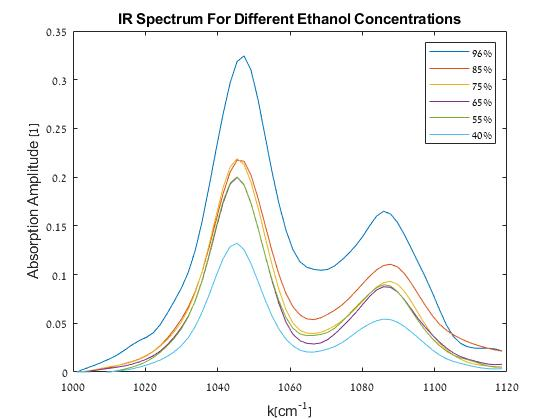
\includegraphics[width=\linewidth]{Images/EthanolAbsorption.jpg}
    \caption{IR spectrum of solutions with different ethanol concentration in the range 1000-1120$cm^{-1}$ }
    \label{fig:EthanolMixtures}
    \centering
\end{figure}

Fitting a linear function according to equation \ref{eq:EthanolLinFit} to the measurements of concentration and absorbance yielded the following (see Figure \ref{fig:EthanolCalibration}).
% need to reference re: fixed
    \begin{figure}[H]
    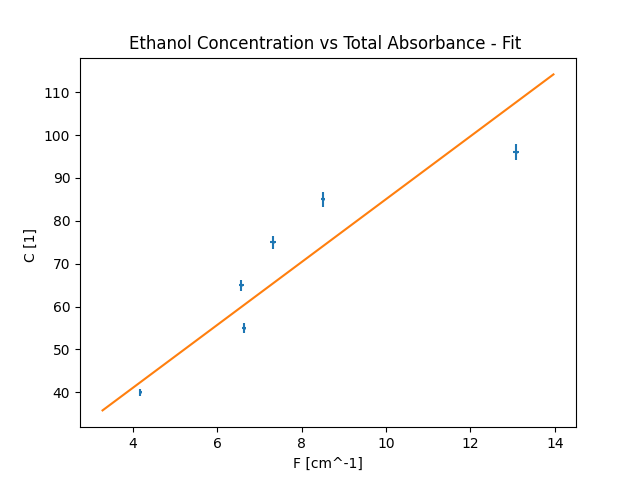
\includegraphics[width=\linewidth]{Images/linear_fittingethanol.png}
    \caption{Linear calibration graph of concentration of ethanol in the solution to total absorbance amplitude in the range $1000-1120 cm^{-1}$}
    \label{fig:EthanolCalibration}
    \centering
\end{figure}
The fit parameters extracted from the linear fit can be seen in Table \ref{ethanol table}.
\begin{table}[H]
    \centering
\begin{tabular}{ |p{2cm}|p{2cm}|p{2cm}|  }
 \hline
 \multicolumn{3}{|c|}{\thead{Fit Parameters and \\Statistical Measures of Ethanol Calibration Graph}} \\ \hline
 Parameter& Value &Error (Relative Error)\\ \hline
 $a_{0}$[$1$]    &$11.7$    &$9.3$($79\%$) \\
 $a_{1}$[$cm$] &$7.3$    & $1.4$ ($19\%$)  \\ \hline
 $P_{value}$ & $3.8\times{10^{-32}}$ & ----- \\ \hline
 $\chi_{red}^2$ & $38$ & ----- \\ \hline
\end{tabular}
\caption{Fit parameters and statistical measures of the ethanol concentration vs absorption amplitude graph}
\label{ethanol table}
\end{table}
$P_{value}$ and $\chi_{red}^2$ are not in their corresponding desirable ranges, more about that in the discussion.
The concentration of ethanol
% Capital E %RE: doesn't have to be capitalized actually. for example in wiki it isn't capitalized mid sentence.
in other solutions was then found by numerically calculating the total absorption in the relevant range and plugging it in the linear equation using the fit parameters. Using the fit parameters from Table \ref{ethanol table} the concentrations in a Suktinis and two unknown alcoholic beverages were found (see Table \ref{beverages table}).
% need to reference tables RE: fixed.
% "Using the fit parameters" is repeated, I think "Table \ref{} shows the calculated concentrations in a Suktinis and two unknown alcoholic beverages", we already said how they were calculated 
%RE: it was explained really briefly in the section regarding ethanol before it and so I wanted to elaborate a bit more.

\begin{table}[H]
\begin{tabular}{ |p{2.8cm}|p{2.8cm}|p{2.8cm}|  }
 \hline
 \multicolumn{3}{|c|}{\thead{Ethanol Concentration in Different Beverages}} \\
 \hline
 Beverage& Concentration(\%) &Concentration Error (Relative Error) \\ \hline
 Suktinis    &$54.3$   &$8.3$ ($15\%$) \\
 Unknown 1  &$40.5$   &$5.7$ ($14\%$) \\
 Unknown 2  &$72$     & $12$ ($17\%$) \\ \hline
\end{tabular}
\caption{Ethanol concentration in different beverages}
\label{beverages table}
\end{table}

\subsection{$\text{CO}_{2}$}
Using the trapezoidal rule
% rule? RE: fixed
 the total absorbance of the air in the region $2270-2400cm^{-1}$ was calculated.
  The total absorbance in that region is proportional to the concentration of $\text{CO}_{2}$ as there are two peaks correlating to $\text{CO}_{2}$ in said region \cite{NISTwebook} and in accordance with equation \ref{eq:BeerLambert}, a linear relation is assumed.
% Use $\text{CO}_{2}$ for $\text{CO}_{2}$ RE: ok
 The ratio between the total absorbance of exhaled air and room air in that region, denoted by $S$, was calculated. $S$  also represents the ratio between $\text{CO}_{2}$ as explained above,
% This sentence is very long. break it up into smaller sentences, like:
% "Using the trapezoidal ??, the total absorbance of the air in the region $2270-2400cm^{-1}$ was calculated. As the total absorbance is closely correlated to the concentration of CO2 in the air, a ratio between the total absorbance of exhaled air and outside (or Tel Aviv) air, denoted by $S$, was calculated. $S$ represents the ratio between CO2 in the air and CO2 in exhaled air RE: integrated some of what you said, what do you think? 
\begin{equation}
\label{eq:CO2ratio}
S=\frac{Absorbance_{Exhaled}}{Absorbance_{Room}}=61\pm24\ (39\%)\ \text{[1]} % Perhaps add \frac{Absorbance_{Exhaled}}{Absorbance_{Outside}}. just writing S is a bit unclear RE:fixed
\end{equation}
$S$
% "This value" to $S$ RE: fixed
would later be
% would later be RE: fixed
compared to that measured a few years ago to see the trend line.  

\subsection{CO}
The absorption peaks from the IR spectrum of CO were extracted and the absorption lines,
% ,
$\Delta T$, 
% ,
and their corresponding angular momentum transitions,
% ,
$m$,
% , RE: fixed all of these
were measured relative to the center point at $\Delta T=2141 cm^{-1}$, $\Delta T$ represents $\Delta J = m = 0 $ and the vibrational transition from $\nu =0$ to $\nu' =1$. Using the locations of the absorption peaks,
% "Using the locations of the absorption peaks, " is clearer RE:fixed
a $3^{rd}$ order polynomial fit was made according to equation \ref{eq:CO_EnrgStatesFit} (see Figure \ref{fig:COPolynomialfit}).
% needs reference RE: fixed
\begin{figure}[H]
    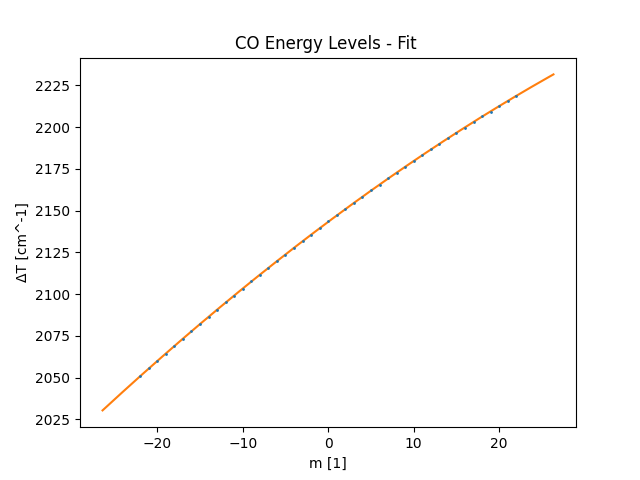
\includegraphics[width=\linewidth]{Images/polynomial_3_fitting.png}
    \caption{$3^{rd}$ order polynomial fit of the spectral lines of the absorption peaks $\Delta T$ as a function of the transition of $CO$'s
    % "the molecule" to "CO" RE: ok
    angular momentum $m$. }
    \label{fig:COPolynomialfit}
    \centering
\end{figure}
The fit parameters and statistical measures extracted can be seen at Table \ref{COfittable}. 
% needs reference RE: fixed
\begin{table}[H]
    \begin{tabular}{ |p{2.8cm}|p{2.8cm}|p{2.8cm}|  }
    
     \hline
     \multicolumn{3}{|c|}{\thead{Fit Parameters and Statistical Measures\\ of the CO absorption lines $3^{rd}$ polynomial fit}} \\
     \hline
     Parameter& Value(\%) & Error (Relative Error) \\ \hline
    $a_{0}[cm^{-1}]$    &$2143.293$  &$0.034$\ ($0.0016\%$) \\
    $a_{1}[cm^{-1}]$  &$3.8220 $  &$0.0040$\  ($0.10\%$) \\
    $a_{2}[cm^{-1}]$  &$-0.01800$     & $1.5\times{10^{-4}}$\ ($0.83\%$) \\ 
    $a_{3}[cm^{-1}]$  &$-9.4\times{10^{-6}}$     & $1.30\times{10^{-5}}$ ($140\%$) \\ \hline
    $P_{value}$ & $0.22$ & ----- \\ \hline
    $\chi_{red}^2$ & $1.2$ & ----- \\ \hline 
    \end{tabular}
    \caption{Fit parameters and statistical measures of the $3^{rd}$ order polynomial fit}
    \label{COfittable}
\end{table}
Using the fit parameters the coefficients in equation \ref{eq:CO_DiffPeturbEnrg} were extracted via the relations stated in equation \ref{eq:COFITcoefficients} (see Table \ref{COcoeftable}).
% needs reference RE: fixed
\begin{table}[H]
    \begin{tabular}{ |p{2.8cm}|p{2.8cm}|p{2.8cm}|  }
    
     \hline
     \multicolumn{3}{|c|}{\thead{Coefficients of The CO Absorption Lines Equation (equation \ref{eq:CO_DiffPeturbEnrg})}} \\
     \hline
     Parameter& Value(\%) & Error (Relative Error) \\ \hline
    $w_{e}[cm^{-1}]$    &$2159.086
    $  &$0.068
    $ ($0.0031\%$) \\
    $x_{e}\ \text{[1]}$  &$0.007315
    $  &$1.6\times{10^{-5}}
    % Gadi said E notation is unclear, we should use 10^{??} instead RE: we should maybe ask gary what he prefers. 
    $  ($0.22\%$) \\
    $B_{e}[cm^{-1}]$  &$1.9290
    $     & $0.0090
    $ ($0.47\%$) \\ 
    $\alpha$ [$cm^{-1}$] & $0.01800
    $ &$1.5\times{10^{-4}}$ ($0.83\%$) \\
    $D_{v}$ [$cm^{-1}$] & $2.4\times{10^{-6}}
    $ & $3.3\times{10^{-6}}$ ($140\%$)
     \\ \hline
    \end{tabular}
    \caption{The coefficients from equation \ref{eq:CO_DiffPeturbEnrg} of the CO absorption lines extracted using the fit parameters}
    \label{COcoeftable}
\end{table}

\subsection{Cigar Smoke's Chemical Makeup Analysis}
By looking at the different peak placements and shapes in the IR absorption spectrum of each cigar's smoke and comparing them to the peaks of chemicals with known peaks in the area from the literature\cite{NISTwebook}, 
% Did you only use that one nist website? RE: are you asking me? if so the answer is no lol
the chemical makeup was found. To aid in this endeavor, past research
% Refrence to papers
on the subject was consulted (See \cite{IRCEllSMOKE} and \cite{FTIRSPECTRAOFSMOKE} in bibliography). The LM00 (as opposed to plain "LM") cigar has the widest range of wave numbers, as such, the LM00 cigar smoke's IR spectrum is shown in Figures \ref{fig:DiverseLM} and \ref{fig:COCO2LM}. Only "(Brand)'s IR spectrum" is written, to be understood as "The (Brand) cigar smoke's IR spectrum". Other IR spectra are quite similar, Galouis and Canadian have the exact same IR spectrum, down to the noise, thus, only Galouis results are shown. NEXT and Marlboro's IR spectra are only between $2000\text{cm}^{-1}$ and $2400\text{cm}^{-1}$ and LM's is between $2000\text{cm}^{-1}$ and $2520\text{cm}^{-1}$, therefore, many substances cannot be identified and quantified.
\begin{figure}[H]
    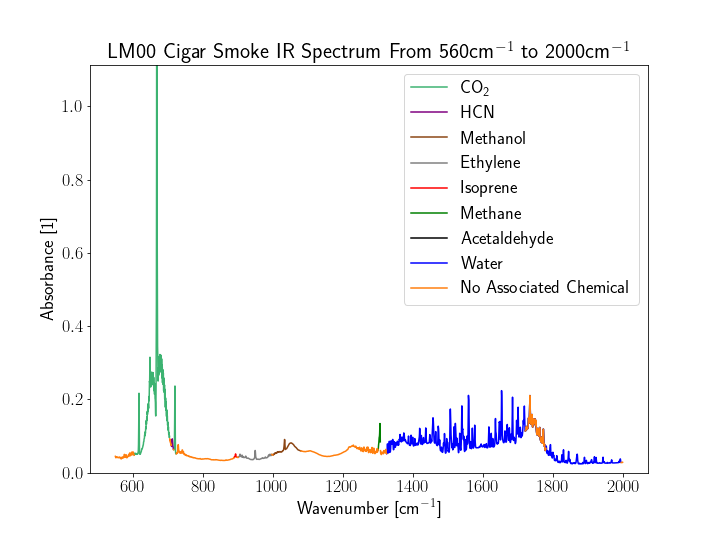
\includegraphics[width=\linewidth]{Images/Colored Cigar Spectrums/LM00_Diverse_Spectrum.png} 
    \caption{IR Spectrum from $560 \text{cm}^{-1}$ to $2000\text{cm}^{-1}$ of LM00 cigar smoke with color-coded regions corresponding to the identifying peaks of each substance.}
    \label{fig:DiverseLM}
\end{figure}
The region from 400$\text{cm}^{-1}$ to 550$\text{cm}^{-1}$ was cut from all measurements as it contains much noise and little identifying peaks.
\begin{figure}[H]
    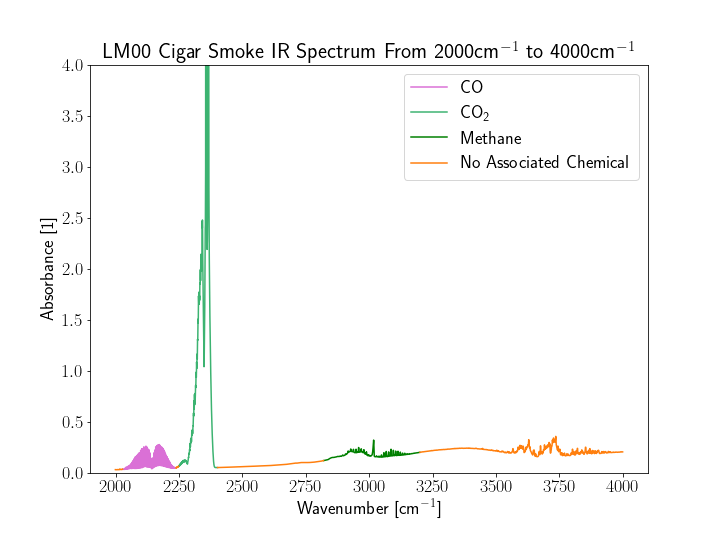
\includegraphics[width=\linewidth]{Images/Colored Cigar Spectrums/LM00_CO-CO2_Spectrum.png} 
    \caption{IR Spectrum from $2000 \text{cm}^{-1}$ to $4000 \text{cm}^{-1}$ of LM00 cigar smoke with color-coded regions corresponding to the identifying peaks of each substance.}
    \label{fig:COCO2LM}
\end{figure}
Note the bumpy area from $3500 \text{cm}^{-1}$ to $4000 \text{cm}^{-1}$, $\text{H}_{2}\text{O}$ and $\text{CO}_{2}$ have been identified in lower wave numbers and this is a mix of the two \cite{FTIRSPECTRAOFSMOKE}.
The area under each substance region was calculated using trapezoidal rule \cite{numerical} 
% reference wikipedia or some paper that shows the method RE: no need.
and is taken as a proxy for substance amount. This metric does not allow for comparison between the substances in a cigar, but does allow for comparison between cigar brands.
The identifying regions for each substance and area for each brand are shown in Tables \ref{tbl:CigarSubstanceRegions} and \ref{tbl:CigarSubstanceAreas}. % ref 

\begin{table}[H]
    \centering
    \begin{tabular}{ |p{2.3cm}|p{3cm}|  }
     \hline
     \multicolumn{2}{|c|}{\thead{Peak Ranges For Substances In Cigar Smoke}} \\ \hline
     Substance & Range\\ \hline
     CO & 2028-2238 $\text{cm}^{-1}$\\ \hline
     $\text{CO}_{2}$ & 604-705 $\text{cm}^{-1}$\newline 717-724 $\text{cm}^{-1}$\newline 2248-2400 $\text{cm}^{-1}$\\ \hline
     HCN & 710-716 $\text{cm}^{-1}$\\ \hline
     Methanol & 1000-1080 $\text{cm}^{-1}$\\ \hline
     Ethylene & 901-997 $\text{cm}^{-1}$\\ \hline
     Isoprene & 889-897 $\text{cm}^{-1}$\\ \hline
     Methane & 1300-1307 $\text{cm}^{-1}$\newline 2820-3200 $\text{cm}^{-1}$\\ \hline
     Acetaldehyde & 1720-1780 $\text{cm}^{-1}$\\ \hline
     $\text{H}_{2}$O & 1325-1994 $\text{cm}^{-1}$\\ \hline
    \end{tabular}
    \caption{Identifying regions for the found substances.}
    \label{tbl:CigarSubstanceRegions}
\end{table}

\begin{table}[H]
    \begin{tabular}{ |p{1.9cm}|p{1.2cm}|p{1.5cm}|p{0.8cm}|p{1.2cm}|p{1.0cm}|  }
     \hline
     \multicolumn{6}{|c|}{\thead{Area Under Identifying Regions For Each Cigar Brand}} \\ \hline
        Substance   & NEXT  & Marlboro & LM    & Galouis   & LM00\\ \hline
        CO          & 18    & 6.6       & 12    & 18        & 22 \\ \hline % is bad with recipts 
     $\text{CO}_{2}$& 180   & 69        & 140   & 170       & 240 \\ \hline
     HCN            & -     & -         & -     & 0.37      & 0.51 \\ \hline % is bad with recipts 
     Methanol       & -     & -         & -     & 4.5       & 4.3 \\ \hline % Makes cigars less harsh and more tasty
     Ethylene       & -     & -         & -     & 3.1       & 3.2 \\ \hline % Irrelevant
     Isoprene       & -     & -         & -     & 0.28      & 0.35 \\ \hline % Possible Carcinogen and is known to influence reproductive and developmental processes in animals
     Methane        & -     & -         & -     & 64        & 91 \\ \hline % Found nothing that states its bad in cigars
     $\text{H}_{2}$O& -     & -         & -     & 43        & 51 \\ \hline
     Acetaldehyde   & -     & -         & -     & -         & - \\ \hline % is bad with recipts 
     Acrolein   & -     & -         & -     & -         & - \\ \hline
     Acetone   & -     & -         & -     & -         & - \\ \hline 
    \end{tabular}
    \caption{Area under the identifying regions of each substance in each brand's smoke.}
    \label{tbl:CigarSubstanceAreas}
\end{table}

Every substance was identified based upon its characteristic absorption lines\cite{NISTwebook}\cite{IRCEllSMOKE}. 
% changed 'using papers cited in the references' to '\cite{}...
Some regions contain multiple absorption lines that overlap, thus restricting the ability to identify the substances that make them up, such as the region of $1300-2000\text{cm}^{-1}$ that contains water's peaks but also many other substances such as acetone, acetaldehyde and acrolein \cite{FTIRSPECTRAOFSMOKE}, which is why acetaldehyde's total absorption could not be estimated. 
NEXT and Marlboro's IR spectra are cut short, only CO and $\text{CO}_{2}$ absorption lines were identified (see Figure \ref{fig:COCO2NEXT}).
As CO and $\text{CO}_{2}$ are present in all smoke spectra a comparison between the different brands is possible. Note that $\text{CO}_{2}$ has absorption lines outside the region $2000-2400 \text{cm}^{-1}$ and thus outside NEXT and Marlboro's IR spectra. As such, the only valid comparison is in the $2000-2400 \text{cm}^{-1}$ region. The ratios of total absorbance between cigars, which according to equation \ref{eq:BeerLambert} is also the ratio between concentrations, was calculated.

\begin{figure}[H]
    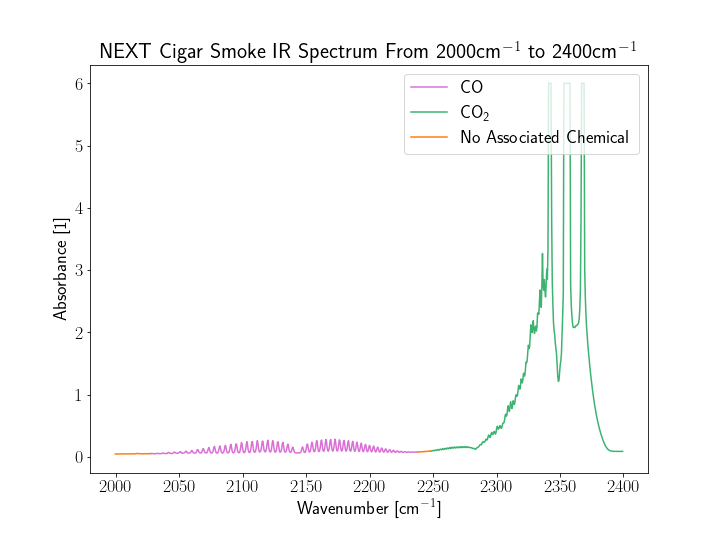
\includegraphics[width=\linewidth]{Images/Colored Cigar Spectrums/NEXT_CO-CO2_Spectrum.png} 
    \caption{IR Spectrum from $2000 \text{cm}^{-1}$ to $2400 \text{cm}^{-1}$ of NEXT cigar smoke with color-coded regions corresponding to the identifying peaks of each substance.}
    \label{fig:COCO2NEXT}
\end{figure}

Calculating the ratios between the total absorbance of $\text{CO}_{2}$ in the region 2248-2400 $\text{cm}^{-1}$ and CO in the region 2028-2238 $\text{cm}^{-1}$ yielded the following ratios (see Table \ref{tbl:CigarCO2RATIOS} and Table \ref{tbl:CigarCORATIOS}). The ratios of $\text{CO}_{2}$ were calculated using outside air as a baseline, whose $\text{CO}_{2}$ total absorption in that region was previously measured. Using the concentration of $\text{CO}_{2}$ in air, $C_{\text{CO}_{2}}=0.041\%$ \cite{NASA}, the concentration of $\text{CO}_{2}$ in the smoke from the cigars was found as well. 

\begin{table}[H]
    \begin{tabular}{ |p{1.9cm}|p{1.2cm}|p{1.5cm}|p{1.4cm}|p{1cm}|p{0.8cm}|  }
     \hline
     \multicolumn{6}{|c|}{\thead{Ratios of $\text{CO}_{2}$ For Different Cigars\\ With Outside Air As A Baseline}} \\ \hline
     Property & NEXT & Marlboro & Galouis & LM00 & LM\\ \hline
     $\text{CO}_{2}$ Ratio & 120 & 44 & 140 & 100 & 83 \\ \hline
     $\text{CO}_{2}$ Concentration &4.9\% & 1.8\%& 5.7\% & 4.1\% & 3.4\% \\\hline
    
    \end{tabular}
    \caption{Ratios of $\text{CO}_{2}$ for different cigars with room air as a baseline.}
    \label{tbl:CigarCO2RATIOS}
\end{table}

The ratios of CO were calculated using the NEXT cigar as the baseline (see Table \ref{tbl:CigarCORATIOS}) since no measurement of CO's IR spectrum in air was made in this experiment.

\begin{table}[H]
    \centering
    \begin{tabular}{ |p{1.5cm}|p{1.5cm}|p{1.5cm}|p{1cm}|  }
     \hline
     \multicolumn{4}{|c|}{\thead{Ratios of CO for Different Cigars}} \\ \hline
      Marlboro & Galouis & LM00 & LM\\ \hline
       0.36 & 1 & 1.2 & 0.82 \\ \hline
    \end{tabular}
    \caption{Ratios of CO for different cigars with NEXT cigar as a baseline.}
    \label{tbl:CigarCORATIOS}
\end{table}

The remaining ratios of gases can only be calculated between the Galouis and LM00 cigars since the other two cigars contain only CO and $\text{CO}_{2}$ absorption lines in their spectrum. These remaining ratios would be referred two in the discussion and can be also calculated directly from Table \ref{tbl:CigarSubstanceAreas}.

\section{Discussion}
\subsection{Thin Polyester Film}
The refractive index of the polyester was found, and the relationship between the sample width and destructive interference frequency was calibrated.
The frequency of each sample was extracted by fitting a sine wave to the area with the clearest sine. For thin (compared to other samples) widths, the region of $2200-2600\ \text{cm}^{-1}$ has particularly clear sine waves.
Other regions of interest are $550-800\ \text{cm}^{-1}$ and $3200-3320\ \text{cm}^{-1}$ which are used when clear enough and the aforementioned region is of little use.
All sine fits are very good apart from that of $24\ \mu m$, whose IR spectrum did not contain a sine but still had a periodicity in the $2200-2600\ \text{cm}^{-1}$ region.
The linear fit between width and frequency is clear, with all points within less than two standard deviations away from the line.
The slope's standard deviation is within accepted levels, and the intercept is less than two standard deviations from its theoretical value.
The extracted widths are interpolated using the calibration. The widths are inline with measured widths.
The extracted refractive index is in the general area of plastics' refractive indices \cite{plasticRefract}. As this is an average over the range of wave lengths in the interferogram, pinpointing which plastic in particular is used is impossible from the refractive index alone. Using the IR spectrum to further narrow down options may be possible, but is out of the scope of this report.

\subsection{Ethanol}
In this part of the experiment we measured the IR spectrum of solutions with different yet 
% drop 'yet'
known ethanol concentrations
% concentrations
and calculated the total absorption amplitude of the solutions in the range $1000-1120 cm^{-1}$ where there are absorption peaks of ethanol. A calibration graph between the concentration of ethanol in the solution and the total absorption amplitude in that range was made using a linear fit according to Beer-Lambert Law from equation \ref{eq:BeerLambert}. 
Using the calibration graph, the concentration of ethanol in different beverages was found. The concentration for Suktinis, $C_{Suktinis}=54.3\pm8.3\ (R.E\ of\ 15\%)$ came out close to the written value of 50\% with $N{\sigma}=0.52$ \cite{Suktinis} which confirms the validity of our calibration to a certain degree. However, as can be seen in figure \ref{fig:EthanolCalibration}
%ref{} - residuals
as well as in table \ref{ethanol table},
% \ref - statistical measures
% I don't understand the reason for the appendix here
the linear fit does not represent the data accurately and that a fit to a polynomial of a $2^{nd}$ degree or higher could have yielded better results. Possible reasons for the somewhat inadequate fit can be that equation \ref{eq:BeerLambert} only holds for low concentrations, whereas 
% where -> whereas
the concentrations
% drop 'used'
in this experiment went as high as 96\%. In addition to that, the absorption peaks of ethanol
% CO2?
have some width, and the total
% total
absorption is calculated
% calculated
for a number of wavelengths in that range, whereas the coefficient in the
% the
Beer-Lambert Law is wavelength dependent and not constant for the entire range.
% I think ', another effect which was not taken into account' is redundent
The consequences of the latter effect can also be seen in figure \ref{fig:EthanolMixtures} where the absorption amplitude changes differently depending on the wavenumbers.
% differently for different wavenumbers. -> depending on the wavenumbers
Regardless, the linear fit did sufficiently well and yielded good results.

\subsection{$\text{CO}_{2}$}
The ratio between the $\text{CO}_{2}$ content of alveolar air (exhaled air) and fresh indoor air (inhaled air) was calculated to be $S_{2020}=61$. This ratio was also calculated for 1998 to be $S_{1998}=72.2\pm1.4$ with the percentage of $\text{CO}_2$ in alveolar air taken to be 5.3\%\cite{bookWithCO2inBreath}, 
%The specific origin of the $\text{CO}_2$ content of Alveolar Air (5.3\%) could not be confirmed and associated with a scientific paper. Thus, $S_{1998}$ may be too low or high, as 5.3\% is a rounded estimate and the real value may be higher or lower.
%, not to mention that the 5.3\% figure may be associated to an earlier year. 
%In addition, i
indoor $\text{CO}_2$ levels had to be approximated conservatively as twice the $\text{CO}_2$ content measured outside, at 730 ppm\cite{tans2009noaa}, this conservative approximation lowers $S_{1998}$ further. Noting both approximations, a downward trend is seen, were this trend to continue indoor and later outdoor $\text{CO}_2$ levels will become too high for comfort or life in the nearing decades (for a more in depth analysis see \cite{Jacobson2019}).

\subsection{CO}
The IR spectrum of CO was measured in the range $2025-2233 cm^{-1}$ where there are absorption lines correlating to the angular momentum and vibrational transitions of the diatomic molecule. The resulting IR spectrum 
% drop 'in that range', we already stated 'IR spectrum of CO was measured in the range $2025-2233 cm^{-1}$'
came out similarly
% ly?
to that described in the literature \cite{jiloEdu}.
There are two symmetrical absorption regions around a center point at $2141cm^{-1}$ with nearly no absorption compared to its surroundings. Using the IR spectrum's absorbance peaks,
% 's peaks (no?)
a $3^{rd}$ order polynomial fit was made according to equation \ref{eq:CO_DiffPeturbEnrg} with $\nu'=1$ as this is the relevant transition in the region measured. The fit validated the theory as can be seen in figure \ref{fig:COPolynomialfit}. This claim is also supported by the statistical measures (see Table \ref{COfittable}) which are within their appropriate regions. Using the fit parameters, the coefficients in equation \ref{eq:CO_DiffPeturbEnrg} were calculated using the relations in
% in
equation \ref{eq:COFITcoefficients}. The coefficients were then compared with their corresponding theoretical values from the literature \cite{jiloEdu}
(see Table \ref{tbl:COTheoreticalValues})
\begin{table}[H]
    \begin{tabular}{ |p{2.3cm}|p{2.8cm}|p{1.0cm}|p{2.0cm}|  }
     \hline
     \multicolumn{4}{|c|}{\thead{Comparison with Theoretical Values \\ of the Coefficients In Equation \ref{eq:CO_DiffPeturbEnrg}}} \\ \hline
     Coefficient & Theoretical Value & $N\sigma$ & Relative Distance \\ \hline
     $D_{v}[cm^{-1}]$ & $6.2\times{10^{-6}}$ & $1.2$ & $61$\% \\ \hline
     $B_{e}[cm^{-1}]$ & $193.13\times{10^{-2}}$ & $3.2$ & $1.5$\%\\ \hline
     $\alpha[cm^{-1}]$ & $1.75\times{10^{-2}}$ & $3.3$ & $5.0$\%\\ \hline
     $w_{e}[cm^{-1]}]$ & $2169.8$ & $160$ & $0.51$\%\\ \hline
     $w_{e}x_{e}[cm^{-1}]$ & $13.29$ & $72$ & $19$\% \\ \hline
    \end{tabular}
    \caption{Comparison of the calculated coefficients with their corresponding theoretical values taken from the literature \cite{jiloEdu}}
    \label{tbl:COTheoreticalValues}
\end{table}
The relative distances were calculated in addition to the calculation of $N\sigma$ as
% since or as
in some cases the relative error of the calculated coefficients was either too small or too big, therefore $N\sigma$ was not indicative of the closeness between the two compared values. Overall the calculated coefficients came out close to the corresponding theoretical ones, with those who are somewhat far sharing the same scale with them. In conclusion, the results are satisfactory and indicate the validity of our model and measurements.

\subsection{IR Spectrum Analysis of The Smoke From Many Cigar Brands}
Many substances were identified, with the aide of past publications, in the IR spectra of the smokes. As some brands' IR spectra only include a limited wave length region, not all substances were identified and quantified in each brand's smoke.
Noting that fact, a comparison between the cigars and the health risks that come with each is made. As most substances were not identified in the brands lacking a wide IR spectrum, a full comparison cannot be made. The comparison is by no means a buyer's guide, as will soon be apparent, cigar smoking is dangerous to life and to be avoided.\\
The harmful effects of each of the identified substances will now be listed. These effects may not necessarily occur for the concentrations in a cigar. As the concentrations were not measured, this report will be based on previous literature on the toxicity of cigars and cigarettes.\\
Starting from the top of Table \ref{tbl:CigarSubstanceAreas}, carbon-monoxide (CO) can take the place of oxygen in blood transport and negatively affect the heart \cite{SubstanceDangerPaper} and dexterity.\\
As stated in PubChem\cite{PubChemCO}: "The first symptoms of carbon monoxide exposure when carboxyhemoglobin (COHb, carbon monoxide taking the place of oxygen in the blood) is 15-30$\%$ are generalized, and may include: headache, dizziness, nausea, fatigue, and impaired manual dexterity. Individuals with ischemic heart disease may suffer from chest pain and decreased exercise duration at COHb levels measured from 1$\%$ - 9$\%$". Cigar smokers have COHb levels ranging from 13\% to 39\% and are reported to experience the above symptoms \cite{COHbInSmokers}.\\
Next up is $\text{CO}_{2}$. As should be obvious, $\text{CO}_{2}$ poisoning can happen, however, no report stating that $\text{CO}_{2}$ poisoning is a risk in cigar smoking under normal circumstances was found. \\
% Other substances such as the aforementioned CO, are a risk sooner than $\text{CO}_{2}$ poisoning can occur.
% Maybe drop this sentence or add citation to CO2 poisoning amounts
After $\text{CO}_{2}$, comes hydrogen cyanide (HCN). HCN can negatively affect the central nervous system, thyroids, lungs and heart \cite{SubstanceDangerPaper}\cite{PubChemHCN}.\\
With a villainous effect on smokers comes methanol. Methanol is added to cigars and cigarettes to "mask unpleasant flavors and harshness of tobacco products, making them easier to start using. Tobacco products with menthol can also be more addictive and harder to quit by enhancing the effects of nicotine" \cite{MethanolFDA}. This flavour also adds to the appeal of tobacco to young adults and teens \cite{MethanolFDA}.\\
Now onto ethylene. As with $\text{CO}_2$, no literature was found that states ethylene is potentially dangerous in cigars.\\
Continuing to isoprene. Isoprene is a possible carcinogen and may be a central nervous system depressant \cite{PubChemIsoprene}.\\
Below isoprene sits methane. As with ethylene, no literature was found which warns of the methane content of cigars and cigarettes. \\
$\text{H}_2\text{O}$ is next up for examination. No literature suggests $\text{H}_2\text{O}$ is of much danger in cigars. \\
Now onto the last three substances, acetaldehyde, acrolein and acetone. While a comparison is not possible, it is of importance to mention their effects. Acetaldehyde is a group 1 carcinogen (meaning it is highly likely to cause cancer) and is the most abundant carcinogen in cigar smoke \cite{AcetaldehydeIARC}\cite{AcetaldehydeInCigars}, it also causes "nasal olfactory epithelial lesions" \cite{SubstanceDangerPaper}.
% 
It is water-soluble, as such, it remains in the smoker's saliva which furthers the exposure. Its origin is partly in the combustion of added sugars that mask the cigar's taste. It has also been shown that acetaldehyde enhances nicotine absorption in rats \cite{AcetaldehydeInRats}, since then, cigarette companies have looked for the optimal ratio of acetaldehyde and nicotine, "based on the results of internal research, Philip Morris increased the level of acetaldehyde in Marlboro cigarettes by 40\% between 1982 and 1992 through the addition of sugars \cite{FortyPercentIncrease}" as stated in \cite{CigarCompaniesInternal}.\\ 
Acrolein in cigar smoke may cause nasal lesions \cite{SubstanceDangerPaper}, and acetone may cause neurological effects \cite{SubstanceDangerPaper}.

Looking at \ref{tbl:CigarSubstanceAreas} and using our newly formed substance toxicity expertise, "LM00" is the worst cigar health-wise as it has the highest CO content, the highest HCN content, is it a close second in methanol and a first in isoprene.

\bibliography{Report}

\end{document}